\documentclass{jfm}

% Compilation
\usepackage{silence} % Silence latex compiler warnings
\WarningFilter{latex}{Command \@xhline has changed} % Filter out warning
  % caused by redefinition between jfm.cls class and array (loaded by
  % siunitx)

% Import custom style file containing common packages and options
\setlength{\paperheight}{\pdfpageheight} % JFM class removes paperheight definition and hyperref raises a warning

% Import custom style file containing common packages and options
\usepackage{preamble}
\graphicspath{{./Figures/}}

% Discrete Fourier Transform
\newcommand{\GenP}{\hat{P}_m}
\newcommand{\POne}{\hat{P}_1}
\newcommand{\PTwo}{\hat{P}_2}
\newcommand{\PThree}{\hat{P}_3}
\newcommand{\PFour}{\hat{P}_4}

% Continuous Fourier Transform
\newcommand{\GenPk}{\hat{P}(\kappa)}
\newcommand{\PZerok}{\hat{P}(0)}

% Define custom math symbols
\DeclareMathOperator{\cn}{Cn}
\DeclareMathOperator{\sgn}{sgn}
\DeclareMathOperator{\Ur}{Ur}
\DeclareMathOperator{\Sk}{Sk}
\DeclareMathOperator{\As}{As}
%\DeclareMathOperator{\Bi}{Bi}

\newcommand{\hilbert}{\mathcal{H}}

% Define custom math functions
\DeclarePairedDelimiter{\round}\lfloor\rceil

% Define \im as Roman i
\newcommand{\im}{\mathrm{i}}
% Replace epsilon with varepsilon
\renewcommand*{\epsilon}{\varepsilon}

%% Use \thalf and \squart commands from JFM class
%\newcommand\squart{\ensuremath{{\textstyle\frac{1}{4}}}}
%\newcommand\thalf{\ensuremath{{\textstyle\frac{1}{2}}}}

\linenumbers

\title{Wind-Induced Changes to Surface Gravity Wave Shape in Shallow Water}

\author{Thomas J. Zdyrski \and Falk Feddersen}

\begin{document}

\maketitle

\begin{abstract}
Wave shape (\eg wave skewness and asymmetry) impacts sediment transport,
beach morphology, and ship safety.
Previous work by the authors showed that wind (via changes in surface
pressure) affects wave shape in intermediate and deep water.
This effect was most pronounced as the depth decreased.
Here, this work investigates the interaction of wind and wave shape in
shallow water.
A multiple-scales analysis is applied to long waves propagating over a
shallow, flat bottom forced by a Jeffreys-type surface pressure.
This produces a Korteweg-de Vries (KdV)-Burgers governing the wave
profile.
The evolution of an initially symmetric solitary wave is calculated
numerically.
The wave's height, skewness, and asymmetry are investigated as functions
of time and pressure magnitude.
The setup's parameters are grouped to form invariant scalings,
providing a simple means of translating between different parameter
ranges.
These results are in qualitative agreement with prior results in
intermediate and deep water.
\end{abstract}

\section{Introduction}

\section{Setup}
\subsection{Governing Equations}
We will treat the flow as irrotational and inviscid throughout the
fluid and neglect surface tension by restricting to wavelengths $\lambda
\gg \SI{2}{\centi\meter}$.
Furthermore, we restrict to planar wave propagation in the $+x$
direction.
Finally, we choose a coordinate system with $z=0$ at the mean water level and
a horizontal, flat bottom located at $z=-h$.
Then, the incompressibility condition and standard boundary conditions
are%
\footnote{
  We used the gauge freedom to absorb the Bernoulli ``constant'' $C(t)$
  in the dynamic boundary condition into the definition of $\phi$.
}
\begin{alignat}{2}
  0 &= \phi_{xx} + \phi_{zz} &&\qq{on}
  -h < z < \eta \,, \label{eq:laplace}\\
  0 &= \phi_{z} &&\qq{on} z=-h \,, \label{eq:bottom_bc}\\
  \phi_{z} &= \eta_{t} + \phi_{x} \eta_{x} &&\qq{on} z = \eta \,,
  \label{eq:kinematic_bc}\\
  \qq*{and} 0 &= \frac{p}{\rho_w} + g\eta + \phi_{t} +
  \frac{1}{2} \bqty{\phi_{x}^2 + \phi_{z}^2} &&\qq{on} z=
  \eta \,. \label{eq:dynamic_bc}
\end{alignat}
Here, $\eta(x,t)$ is the wave profile, $\phi(x,z,t)$ is the velocity
potential $\vec{u} = \grad{\phi}$, $p(x,t)$ is the surface pressure,
$g$ is the acceleration due to gravity, and $\rho_w$ is the water
density.
We are seeking a spatially-periodic progressive wave:
\begin{gather}
  \eta(\vec{x},t) = \eta(x + \lambda, t) \,,
\end{gather}
with similar conditions on $\vec{u}$.
We are parameterizing our initial wave by four dimensional quantities:
the mean depth, bottom horizontal velocity, wave height, and wavelength.
We will choose a coordinate system where the average bottom horizontal
velocity vanishes:
\begin{equation}
  \overline{ \pdv{\phi}{x} } = 0 \qq{on} z=-h \,,
  \label{eq:bot_bc_horz}
\end{equation}
with the overline an average over a wavelength.
Additionally, we assume the surface pressure $p(x,t)$ is given by a
Jeffreys-type forcing \citep{jeffreys1925formation}:
\begin{equation}
  p(x,t) = P \pdv{\eta(x,t)}{x} \,.
\end{equation}
Here, $P$ is proportional to $(U-c)^2$, with $U$ the wind speed and $c$
the wave speed (\cf \cref{sec:press_mag}), and $P>0$ corresponding to wind in
the same direction as the wave.

\subsection{Nondimensionalization}
We will normalize by identifying characteristic scales.
The parameters we know \apriori are the characteristic horizontal length
scale $L$ over which $\eta$ changes rapidly, the (initial) wave height
$H_0$, the depth $h$, the gravitational acceleration $g$, and the wind
speed $U$ expressed as a pressure magnitude $P \propto \rho_a (U-c)^2$.
However, instead of using $L$, we will instead use an effective
wavenumber $k_E \coloneqq 2 \pi/ L$.
Denoting nondimensional variables with an prime, we have
\begin{equation*}
  \begin{aligned}
  x &= \frac{x'}{k_E} = h \frac{x'}{\sqrt{\mu}}\,, \\
  z &= h z' \,,
  \end{aligned}
  \qquad
  \begin{aligned}
  t &= \frac{t'}{k_E\sqrt{g h}}
    = \frac{t'}{\sqrt{\mu}} \sqrt{\frac{h}{g}} \,, \\
  P &= \epsilon P' \frac{\rho_w g}{k_E}
    = \frac{\epsilon}{\sqrt{\mu}} P' \rho_w g h \,,
  \end{aligned}
  \qquad
  \begin{aligned}
  \eta &= a_0 \eta' = h \epsilon \eta' \,, \\
  \phi &= \phi'\frac{a_0}{k_E}\sqrt{\frac{g}{h}}
    = \frac{\phi'\epsilon}{\sqrt{\mu}}\sqrt{g h^3} \,,
  \end{aligned}
\end{equation*}
with $a_0 \coloneqq H_0/2$ the initial wave amplitude.
Here, we have defined the parameters $\epsilon \coloneqq H_0/(2h)$ and $\mu
\coloneqq (kh)^2$, while choosing $\order{P k_E/(\rho_w g)} =
\order{\epsilon}$.
Our problem is defined by these three small, nondimensional parameters.
We will later require that $\order{\epsilon} = \order{\mu}$.
Furthermore, we see that $\epsilon/\mu$ is proportional to the Ursell
number, $\Ur = H \lambda^2/h^3 = 8 \pi^2 \epsilon/\mu$.
Using these definitions, our equations take the form
\begin{alignat}{2}
  0 &= \mu \phi'_{x'x'} + \phi'_{z'z'} &&\qq{on}
    -1 < z' < \epsilon \eta' \,, \label{eq:laplace_nondim} \\
  0 &= \phi'_{z'} &&\qq{on} z'=-1 \,, \label{eq:bottom_bc_nondim} \\
  \phi'_{z'} &= \mu \eta'_{t'} +
    \epsilon \mu \phi'_{x'} \eta'_{x'} &&\qq{on} z' = \epsilon \eta' \,,
    \label{eq:kinematic_bc_nondim} \\
  0 &= \epsilon P' \eta'_{x'} +  \eta' + \phi'_{t'} + \frac{1}{2}
    \pqty{\epsilon \phi_{x'}^{\prime \, 2} + \frac{\epsilon}{\mu}
    \phi_{z'}^{\prime \, 2}} &&\qq{on} z'= \epsilon \eta' \,.
    \label{eq:dynamic_bc_nondim}
\end{alignat}
Note that this is equivalent to choosing a set of units wherein $h = g =
\rho_w = 1$.
The primes will be dropped henceforth for readability.

\subsection{Depth Dependence of \texorpdfstring{$\phi$}{Velocity Potential}}
Here, we will reproduce the Bousinesq derivations provided by
\citet{mei2005nonlinear}, modified to include a surface pressure
forcing.
The depth dependence of $\phi$ can be determined from Laplace's equation
\cref{eq:laplace_nondim} and the bottom boundary condition
\cref{eq:bottom_bc_nondim}.
We will do this be expanding $\phi$ in a Taylor series about the bottom
$z=-1$:
\begin{equation}
  \phi(x,y,z,t) = \sum_{n=0}^\infty (z+1)^n\phi_n(x,y,t) \,.
\end{equation}
A standard calculation \citep[\eg][]{mei2005nonlinear} yields $\phi$
as a partial expansion of $\phi$ in terms of $\mu$:
\begin{equation}
  \phi(x,z,t) = \sum_{n=0}^{\infty} (-\mu)^n \frac{(z+1)^{2n}}{(2n)!}
  \partial_x^{2n} \phi_0(x,t; \mu, \epsilon) \,.
  \label{eq:phi_expansion}
\end{equation}
If we assume $\mu \ll 1$, we have,
\begin{equation}
  \phi = \phi_0 - \frac{1}{2}\mu (z+1)^2\partial^2_x\phi_0 +
  \frac{\mu^2}{24}(z+1)^4\partial^4_x\phi_0 +
  \order{\mu^3} \,.
\end{equation}
Note that truncating our series $\phi_n$ at finite $n$ means
Laplace's equation is only satisfied approximately.
For convenience, we will define $\varphi \coloneqq \phi_0$, as we will
need to append more subscripts shortly.

Now, our goal is to determine the form of $\eta$ and $\varphi$.
Substituting this series expansion into the two
remaining boundary equations,
\cref{eq:kinematic_bc_nondim,eq:dynamic_bc_nondim} and recalling that
they are evaluated at $z=\epsilon \eta$, we have reduced our system to
the Boussinesq equations with a pressure forcing term,
\begin{gather}
  \eta_t + \pqty{H\varphi_x}_x
    -\frac{1}{6}\mu \pqty{H^3\varphi_{xxx}}_x =
    \order{\mu^2} \label{eq:kinematic_bc_varphi} \,, \\
  \epsilon P \eta_x + \eta + \varphi_t - \frac{1}{2}\mu H^2\varphi_{txx} +
    \frac{1}{2}\epsilon\pqty{\varphi_x}^2 = \order{\mu^2} \,,
  \label{eq:dynamic_bc_varphi}
\end{gather}
where subscripts denote partial derivatives.
Note that we have used the total depth $H\coloneqq 1+\epsilon\eta$.
Further, we will now assume $\order{\epsilon} = \order{\mu} \ll 1$ which
implies $\Ur = \order{1}$.

\subsection{Perturbation Expansion}
\label{sec:shallow_water}
We expand our timescale in terms of multiple timescales $t_n =
\epsilon^n t$ for $n= 0,1,2,\ldots$.
Thus, all time derivative become $\partial_t \to \partial_{t_0} +
\epsilon \partial_{t_1} + \ldots$.
Then, we expand our variables in an asymptotic series of $\mu$
\begin{align}
  \eta(x,t) &= \sum_{k=0}^{\infty} \epsilon^k
    \eta_{k+1}(x,t_0,t_1,\ldots) \,, \\
  \varphi(x,t) &= \sum_{k=0}^{\infty} \epsilon^k
    \varphi_{k+1}(x,t_0,t_1,\ldots) \,.
\end{align}

\section{Derivation of KdV-Burgers Equation}
Now, we will reduce the Bousinessq equations
\cref{eq:kinematic_bc_varphi,eq:dynamic_bc_varphi} to the KdV equations.
\subsection{Zeroth Order Equations}
Collecting order-one terms $\order{\epsilon^0}$ from
\cref{eq:kinematic_bc_varphi,eq:dynamic_bc_varphi} gives
\begin{gather}
  \pdv{\eta_0}{t_0} + \pdv[2]{\varphi_0}{x} = 0 \,, \\
  \eta_0 + \pdv{\varphi_0}{t_0} = 0 \,.
\end{gather}
Eliminating $\eta_1$ from this gives
\begin{equation}
  \pqty{\pdv[2]{t_0} - \pdv[2]{x} } \varphi_0 = 0 \,.
  \label{eq:wave_eq}
\end{equation}
This is the standard one-dimensional wave equation.
This implies
\begin{equation}
  \varphi_0 = f_0(x-t_0,t_1) + g_0(x+t_0,t_1) \,.
  \label{eq:phi0_sol}
\end{equation}
Here, we have neglected the term linear in $t_0$ since we already set
our gauge condition $\varphi = f(t_0)$, and we neglected the term linear
in $x$ since we have chosen \cref{eq:bot_bc_horz} that $u =
\pdv*{\varphi}_x = 0$ at the bottom.
We will restrict to right-moving waves and take $g_0 = 0$.
This also gives
\begin{equation}
  \eta_0 = - \pdv{\varphi_0}{t_0} = f_0'(x-t_0,t_1) \,,
  \label{eq:eta0_sol}
\end{equation}
with $f_0'(x-t_0,t_1) \coloneqq \eval{\pdv*{\theta}
f_0(\theta,t_1)}_{\theta = x-t_0}$.

\subsection{\label{sec:int_first_order} First Order Equations}
Continuing to the next order of perturbation theory, we retain terms of
order $\order{\epsilon}$.
Inserting our previous solutions, \cref{eq:phi0_sol,eq:eta0_sol} yields
\begin{gather}
  \begin{aligned}
    \pdv{\eta_1}{t_0} + \pdv[2]{\varphi_{1}}{x} &=
      -\pdv{\eta_0}{t_1} - \pdv{x} \pqty{\eta_0 \pdv{\varphi_0}{x}} +
      \frac{1}{6} \frac{\mu}{\epsilon} \pdv[4]{\varphi_0}{x} \\
      &= -\pdv{f_0'}{t_1} - 2 f_0' f_0'' + \frac{1}{6}
      \frac{\mu}{\epsilon} f_0^{(4)} \,,
  \end{aligned}
  \\
  \begin{aligned}
    \eta_1 + \pdv{\varphi_1}{t_0} &= -P \pdv{\eta_0}{x} -\pdv{\varphi_0}{t_1}
      + \frac{1}{2} \frac{\mu}{\epsilon} \frac{\partial^3 \varphi_0}
        {\partial t_0 \partial^2 x}
      - \frac{1}{2} \pqty{ \pdv{\varphi_0}{x} }^2 \\
    &= -\pdv{f_0}{t_1} - P \pdv{\eta_0}{x} - \frac{1}{2} \frac{\mu}{\epsilon}
      f_0^{(3)} - \frac{1}{2} \pqty{f_0'}^2 \,,
  \end{aligned}
\end{gather}
with $f_0^{(n)} \coloneqq \eval{\pdv*[n]{\theta}
f_0(\theta,t_1)}_{\theta=x-t_0}$ the $n$-th derivative of $f_0$.

We can eliminate $\eta_1$ from these equations to give
\begin{equation}
  \pqty{\pdv[2]{x} - \pdv[2]{t_0}} \varphi_1 = -2 \pdv{f_0'}{t_1} +
    P\pdv{\eta_0}{t_0}{x} - 3 f_0' f_0'' - \frac{1}{3} \frac{\mu}{\epsilon}
    f_0^{(4)} \,.
\end{equation}
However, we assume all order $\varphi_{n}$ travel at the same speed; in
particular, this means we will choose
\begin{align}
  \varphi_1 = f_1(x-t_0,t_1,\ldots) \,, \label{eq:phi1_sol} \\
  \eta_1 = f_1'(x-t_0,t_1,\ldots) \,. \label{eq:eta1_sol}
\end{align}
Thus, the left hand side vanishes:
\begin{equation}
  \pdv{f_0'}{t_1} + \frac{1}{2} P f^{(3)} + \frac{3}{2} f_0' f_0''
    + \frac{1}{6} \frac{\mu}{\epsilon} f_0^{(4)} = 0\,.
\end{equation}
Converting back to $\eta_0$ gives
\begin{equation}
  \pdv{\eta_0}{t_1} + \frac{3}{2}
    \eta_0 \pdv{\eta_0}{x} + \frac{1}{6} \frac{\mu}{\epsilon}
    \pdv[3]{\eta_0}{x} = -P \frac{1}{2} \pdv[2]{\eta_0}{x} \,.
  \label{eq:kdv_burgers}
\end{equation}
This is the Korteweg-de Vries (KdV)-Burgers equation, though the
``damping term'', $\partial^2_x \eta_0$ can have a ``negative
viscosity'' (which is expected, since the wind should cause growth
rather than decay).
The KdV-Burgers equation is not known to have any closed form solutions,
so we will instead solve this numerically.

\section{Initial Conditions}
For an initial condition, we will choose the solutions of the ordinary
KdV equation: cnoidal or solitary waves (which are a special case of
cnoidal waves).
The general case of the KdV equation, with arbitrary coefficients, is
\begin{equation}
  \mathcal{A} \pdv{\eta_0}{t_1} + \mathcal{F} \pdv{\eta_0}{x} + \mathcal{B}
  \eta_0 \pdv{\eta_0}{x} + \mathcal{C} \pdv[3]{\eta_0}{x} = 0 \,.
\end{equation}
Using the solution from \citet{dingemans1997water} (as quoted in
\citealp{brun2018convective}) and rescaling variables, the solitary
wave solution is
\begin{equation}
  \eta_0 = H_0 \sech^2\pqty{\frac{x - c_1 t_1}{\Delta}} \,,
\end{equation}
with
\begin{equation}
  \Delta = \sqrt{\frac{12 \mathcal{C}}{\mathcal{B}} \frac{1}{H_0}}
  \qq{and}
  c_1 = \frac{\mathcal{F}}{\mathcal{A}} + \frac{H_0 \mathcal{B}}{3
    \mathcal{A}} \,.
\end{equation}
Here, $\abs{H_0}$ is an order-1 parameter and $\sgn(H_0) =
\sgn(\mathcal{B} \mathcal{C})$.
For our particular system, we have $\mathcal{A} = 1$, $\mathcal{B} =
3/2$, $\mathcal{C} = \mu/(6\epsilon)$, and $\mathcal{F} = 0$.

\subsection{Value of Nondimensional Parameters}
If we temporarily revert back to dimensional variables (with primes
denoting dimensionless), we have
\begin{equation}
  \begin{split}
  \frac{\eta_0}{\epsilon h} &= H'_0 \sech^2\pqty{\frac{k_E x - k_E
    \sqrt{gh} c_1' \epsilon t}{\Delta'}}
  \\
  \implies
  \eta_0 &= \epsilon h H'_0
  \sech^2\pqty{\frac{k_E}{\Delta'} \bqty{x - \epsilon \sqrt{gh} c_1' t}}
  \\
  &\coloneqq H_0 \sech^2\pqty{\frac{x - c_1 t}{\Delta}} \,.
  \end{split}
\end{equation}
Here, we have defined the dimensional quantities $H_0$, $\Delta$, and $c_1$:
\begin{gather}
  H_0 = \epsilon h H'_0
  \qq{and}
  \Delta = \frac{\Delta'}{k_E}
  \label{eq:nondim_solitary_params}
  \\
  \qq{and}
  c_1 = \epsilon \sqrt{gh} c_1' = \epsilon \sqrt{gh} \pqty{
    \frac{\mathcal{F}}{\mathcal{A}} +
    \frac{\mathcal{B} H_0}{3 \mathcal{A}} }
\end{gather}
Given the conventional definition that $H_0 = 2 a_0$, we have
\begin{equation}
  2 a_0 = \epsilon h H'_0 = a H'_0 \implies H'_0 = 2 \,.
\end{equation}
We choose
\begin{equation}
  k_E \coloneqq \frac{2}{\Delta}
\end{equation}

Finally, we can now fix $\mu$ as a function of $\epsilon$:
\begin{equation}
  k_E = \frac{2}{\Delta} = \frac{2 k_E}{\Delta'}
  \implies \Delta' = 2 \,.
\end{equation}
However, using \cref{eq:nondim_solitary_params}, we have
\begin{equation}
  2 = \Delta ' = \sqrt{\frac{12 \mathcal{C}}{\mathcal{B}}
    \frac{1}{H'_0}}
  = \sqrt{\frac{12 \mathcal{C}}{\mathcal{B}} \frac{1}{2}}
  \implies 1 = \frac{2 \mathcal{B}}{3 \mathcal{C}} \,.
\end{equation}
For our particular values of $\mathcal{B} = 3/2$ and $\mathcal{C} =
\mu/(6 \epsilon)$, we have
\begin{equation}
  1 = 6 \frac{\epsilon}{\mu} \,.
\end{equation}
This means that we have the requirement that
\begin{equation}
  \mu = 6 \epsilon
\end{equation}
for solitary waves.
This is simply the well-known fact that the height and width of a
solitary wave satisfy a fixed relationship.

Therefore, the nondimensional equation we are solving is
\begin{equation}
  \mathcal{A} \pdv{\eta'_0}{t'_1} + \mathcal{F} \pdv{\eta'_0}{x'} + \mathcal{B}
  \eta'_0 \pdv{\eta'_0}{x'} + \mathcal{C} \pdv[3]{\eta'_0}{{x'}} =
  \mathcal{G} \pdv[2]{\eta'_0}{{x'}} \,.
  \label{eq:kdvb_nondim}
\end{equation}
with $\mathcal{A} = 1$, $\mathcal{B} = 3/2$, $\mathcal{C} = 1$, and
$\mathcal{G} = -P'/2$.
We wish for the unforced case to be stationary in this frame of
reference, so we include an $\mathcal{F}$ term such that the unforced
phase speed $\eval{c_1}_{P=0} = 0$:
\begin{equation}
  \mathcal{F} = -\frac{4}{3} \mathcal{B} \,.
\end{equation}
Note that this is equivalent to boosting to a frame moving with the
unforced phase speed.
For our initial condition, we use
\begin{equation}
  \eta'_0(x) = 2 \sech^2\pqty{\frac{x'}{2}} \,.
  \label{eq:initial_cond_nondim}
\end{equation}

\section{Numerics}
To solve \cref{eq:kdvb_nondim} subject to the initial condition
\cref{eq:initial_cond_nondim}, we will use numerical methods.
The spatial domain has periodic boundary conditions and $N_x = 400$
points spread over a domain of length $L'_x = 20$.
This yields a spacing $\Delta x' = 0.05$, with $x' = 0, \Delta x',
2\Delta x', \ldots L'_x - \Delta x'$.
The simulation is run for from $t'= 0$ to $L'_t = 4$, inclusive, with
$N_t = \num{6.4e5}$ points, yielding a spacing $\Delta t' = L'_t/(N_t-1)
\approx \num{6.25e-6}$.

The PDE \cref{eq:kdvb_nondim} is discretized in space using a
second-order central finite difference method and in space using a
\nth{3}-order Runge-Kutta scheme.
For numerical stability, we must also include a hyperviscosity term
$\mathcal{H}$,
\begin{equation}
  \mathcal{A} \pdv{\eta'_0}{t'_1} + \mathcal{F} \pdv{\eta'_0}{x'} + \mathcal{B}
  \eta'_0 \pdv{\eta'_0}{x'} + \mathcal{C} \pdv[3]{\eta'_0}{{x'}} =
  \mathcal{G} \pdv[2]{\eta'_0}{{x'}} - \mathcal{H}
  \pdv[4]{\eta'_0}{{x'}} \,,
\end{equation}
with $\mathcal{H} = \num{3e-3}$.

\section{Results}
Given the one free parameter $P k_E/(\rho_w g \epsilon)$ of the
KdV-Burgers equation \cref{eq:kdvb_nondim}, we can now plot the results
for different $P k_E/(\rho_w g \epsilon)$.
In particular, we are interested in different values of $\sgn(P)$:
recall that $P>0$ ($P<0$) implies wind in the same (opposite) direction
as the waves.

\begin{figure}
  \centering
  { % Put \phantomsubcaption in their own group to prevent it from
    % affecting the main figure's numbering
    \phantomsubcaption
    \label{fig:snapshots_solitary:a}
    \phantomsubcaption
    \label{fig:snapshots_solitary:b}
  }
  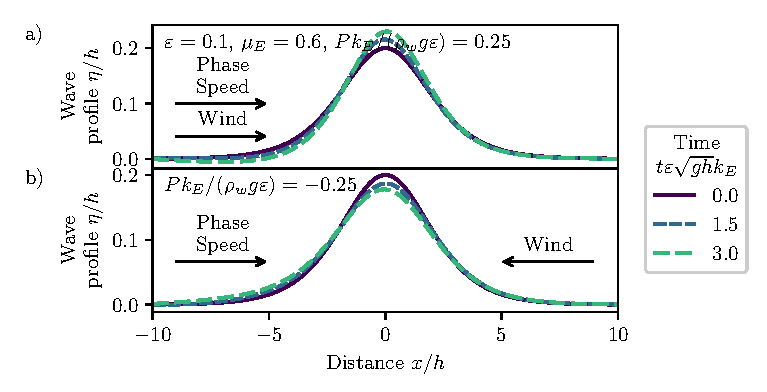
\includegraphics{Snapshots-Positive-Negative.eps}
  \caption{
    Evolution of a solitary wave profile under
    \subref{fig:snapshots_solitary:a}
    onshore and
    \subref{fig:snapshots_solitary:b}
    offshore Jeffreys forcing.
    The nondimensional wave height $\eta/h$ is plotted for
    nondimensional distance $-10 \le x/h \le 10$.
    Results are shown for $\epsilon=0.1$, $\mu_E = 0.6$, and $\abs{P
    k_E/(\rho_w g \epsilon)} = 0.25$ nondimensional slow times $t
    \epsilon \sqrt{gh} k_E = 0$, $2$, and $4$, as indicated in the
    legend.
    The arrows denote the direction of wave propagation (phase speed) or
    wind direction.
  }
  \label{fig:snapshots_solitary}
\end{figure}

In \cref{fig:snapshots_solitary}, we have plotted the wave profile
$\eta/h$ as a function of distance $x/h$ at different nondimensional
slow times $t \epsilon \sqrt{g h} k_E$ and wind directions.
Both cases are plotted for initial wave steepness $\epsilon = 0.1$ and
pressure magnitude $\abs{P k_E/(\rho_w g \epsilon)} = 0.25$; the onshore
wind \subref{fig:snapshots_solitary:a} corresponds to $P>0$ while the
offshore wind \subref{fig:snapshots_solitary:b} has $P<0$.
We see that the initially symmetric solitary wave evolving over time
under the influence of \subref{fig:snapshots_solitary:a} onshore and
\subref{fig:snapshots_solitary:b} offshore winds.
For the onshore case \subref{fig:snapshots_solitary:a}, the wave grows,
steepens, and pitches forward, while the wave decays, becomes less
steep, and pitches backwards for the offshore case
\subref{fig:snapshots_solitary:b}.

\begin{figure}
  \centering
  { % Put \phantomsubcaption in their own group to prevent it from
    % affecting the main figure's numbering
    \phantomsubcaption
    \label{fig:statistics_solitary:a}
    \phantomsubcaption
    \label{fig:statistics_solitary:b}
    \phantomsubcaption
    \label{fig:statistics_solitary:c}
  }
  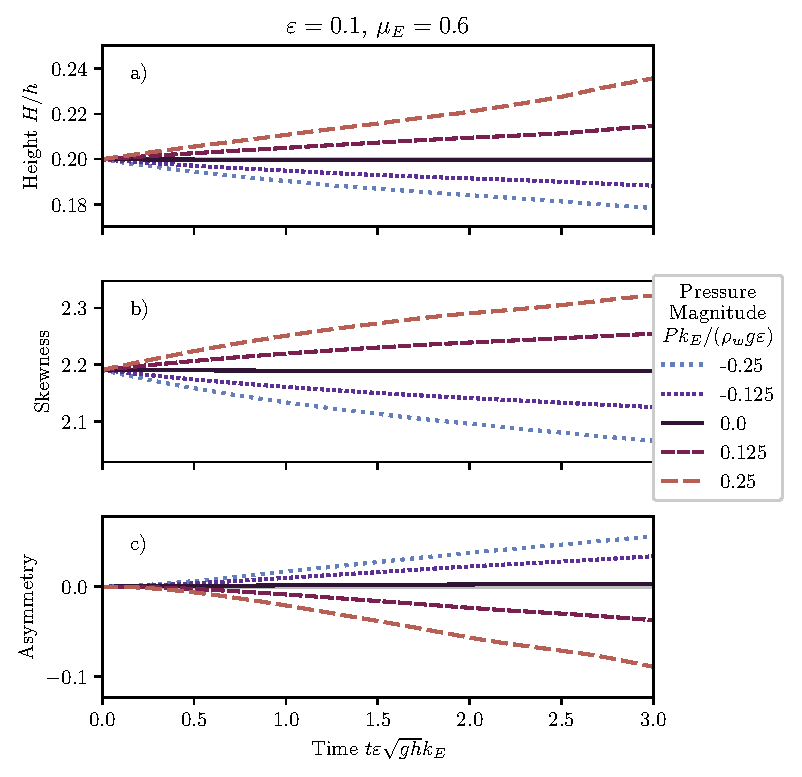
\includegraphics{Skew-Asymm-No-Peak.eps}
  \caption{
    Shape statistics of a solitary profile under onshore and offshore
    Jeffreys forcing are shown for nondimensional slow time $t \epsilon
    \sqrt{gh} k_E \numrange{0}{4}$.
    The
    \subref{fig:statistics_solitary:a}
    height,
    \subref{fig:statistics_solitary:b}
    skewness, and
    \subref{fig:statistics_solitary:c}
    asymmetry are defined in
    \cref{eq:height_def,eq:skew_def,eq:asym_def}.
    Results are shown for $\epsilon=0.1$, $\mu_E = 0.6$, and $P
    k_E/(\rho_w g \epsilon) = 0$, $\pm 0.125$, and $\pm 0.25$, as
    indicated in the legend.
    The solid black line corresponds to the unforced case, $P = 0$, and
    shows no growth or asymmetry and a constant, positive skewness.
  }
  \label{fig:statistics_solitary}
\end{figure}

We have plotted various shape statistics for the solitary wave in
\cref{fig:statistics_solitary} as functions of the nondimensional slow
time $t \epsilon \sqrt{g h} k_E$.
The \subref{fig:statistics_solitary:a} wave height is calculated as
\begin{equation}
  H(t) = \max{\eta} - \min{\eta} \,.
  \label{eq:height_def}
\end{equation}
Wave shape can be quantified by the third-order moments, skewness and
asymmetry.
The \subref{fig:statistics_solitary:b} skewness is defined as
\begin{equation}
  \Sk \coloneqq \frac{\langle \eta^3 \rangle}{\langle \eta^2
  \rangle^{3/2}} \,,
  \label{eq:skew_def}
\end{equation}
and the \subref{fig:statistics_solitary:c} asymmetry is defined as
\begin{equation}
  \As \coloneqq \frac{\langle \hilbert \Bqty{\eta^3} \rangle}{\langle
    \eta^2 \rangle^{3/2}} \,,
  \label{eq:asym_def}
\end{equation}
with $\hilbert$ the Hilbert transform and
\begin{equation}
  \langle f \rangle \coloneqq \frac{1}{L'_x} \int_{-L'_x/2}^{L'_x/2} f
  \dd{x} \,.
\end{equation}
Additionally, each statistic is plotted for onshore wind ($P
k_E/(\rho_w g \epsilon) = 0.125$ and $0.25$), offshore wind ($P
k_E/(\rho_w g \epsilon) = -0.125$ and $-0.25$), and the unforced case
($P k_E/(\rho_w g \epsilon) = 0$).
All cases are plotted for initial steepness $\epsilon = 0.1$ up to slow
time $t'_1 = 3$, corresponding to $3/\epsilon = 30$ wave periods.
The height \subref{fig:statistics_solitary:a} begins at $H_0/h = 2
\epsilon = 0.2$ and shows the onshore wind
causing wave growth while the offshore wind causes decay, as was
observed in \cref{fig:snapshots_solitary}.
The skewness of the initial profile is \num{2.19}, with onshore
(offshore) causing the wave to become more (less) skewed over time.
Finally, the initial profile has zero asymmetry, and the unforced case
$P=0$ maintains zero asymmetry over time.
However, the onshore wind causes the asymmetry to become negative
corresponding to a tilting backwards, while the offshore wind increases
the asymmetry causing the wave to tilt forwards, as seen in
\cref{fig:snapshots_solitary}.

\section{Discussion}

\subsection{\label{sec:press_mag} Pressure Magnitude Estimation}
Now, we will estimate the wind speeds associated with different pressure
magnitudes $P$ over a simple sinusoidal wave.
In \cref{sec:energy_growth_rate}, we show that Jeffreys forcing yields
an energy growth rate
\begin{equation}
  \frac{\gamma}{\omega_0} = \frac{P k}{\rho_w g} \,,
  \label{eq:growth_rate_P}
\end{equation}
with $\omega_0$ the unforced angular frequency.
According to \citet{donelan2006wave}, the wind speed and growth rate
are related in shallow water by
\begin{equation}
  \frac{\gamma}{\omega_0} = \frac{\rho_a}{\rho_w} (ak)
  \pqty{\frac{U_{\lambda/2}}{c_0} - 1}^2
  G \bqty{(ak)
  \pqty{\frac{U_{\lambda/2}}{c_0} - 1}^2}
  \label{eq:growth_rate_U}
\end{equation}
with $G[x] = b - q \mathcal{H}(x - 1)$ with $b = 4.91$, $q = 3.98$, and
$\mathcal{H}$ the Heaviside unit step function.
Furthermore, in the logarithmic boundary layer, we have
\begin{equation}
  \frac{U_z}{\ln(z/z_0)} = \text{const}
  \implies U_{z} = U_{\lambda/2} \frac{\ln(z/z_0)}{\ln[\lambda/(2 z_0)]}
  \label{eq:log_boundary_layer}
\end{equation}
with \citep{taylor2001dependence}
\begin{equation}
  \frac{z_0}{H} = 1200 \pqty{\frac{H}{\lambda}}^{4.5}
\end{equation}
where $H$ is the wave height.
Using \cref{eq:growth_rate_P,eq:growth_rate_U,eq:log_boundary_layer}, we
can calculate the pressure magnitude $P$ from the wind speed $U$ at an
arbitrary height.
If we take $\rho_a/\rho_w = \num{1.225e-3}$, $\mu = \epsilon = 0.1$, $T
= \SI{10}{\second}$, $h = \SI{10}{\meter}$, and $U_{10} =
\SI{50}{\meter\per\second}$ gives $P k_E/(\rho_w g) = \num{4.6e-3} \approx
\epsilon^2$.
If we instead consider laboratory conditions with $h=\SI{0.37}{\meter}$,
$\mu = 1.4$, $\epsilon = 0.14$, and $U_{0.3} = \SI{8}{\meter\per\second}$
as in \citet{feddersen2005wind}, we instead get $P k_E/(\rho_w g) =
\num{4.5e-3} \approx \epsilon^3$.

\subsection{Nondimensional Parameters}
The two dependent variables $\eta'$ and $\varphi'$ of our system
\cref{eq:kinematic_bc_varphi,eq:dynamic_bc_varphi} are controlled by a
number of nondimensional variables and parameters: $x'$, $t'_0$, $t'_1$,
$\epsilon$, $\mu$, and $P'$.
The Buckingham Pi theorem implies that $\eta'$ has the following
dependence
\begin{equation}
  \eta' = f(x', t'_0, t'_1, \epsilon, \mu, P') \,.
\end{equation}
A similar result holds for $\varphi'$, but we are mainly interested in
$\eta'$.
Seeking right-propagating waves at leading order gives
\begin{equation}
  \eta' = f(x'-t'_0, t'_1, \epsilon, \mu, P') \,.
\end{equation}
However, \cref{eq:kdv_burgers} shows $\epsilon$ and $\mu$ only enter as
the quotient $\mu/\epsilon \propto \Ur^{-1}$:
\begin{equation}
  \eta' = f(x'-t'_0, t'_1, \Ur, P') \,.
  \label{eq:kdvb_sol_buckingham}
\end{equation}
By choosing solitary waves as our initial condition, we fixed $\Ur
4\pi^2/3$.

For the unforced KdV equation, $P'=0$, so
\begin{equation}
  \eval{\eta'}_{P'=0} = f('x - t'_0, t'_1) \,.
\end{equation}
In fact, since the KdV equation supports traveling waves, we can
restrict even more to
\begin{equation}
  \eval{\eta'}_{P'=0} = f(x'-c' t') \,,
\end{equation}
with $c' = 1 + \epsilon c_1'$.
This simply expressed the well-known fact that, though solitary KdV
waves are controlled by a single factor parameter $H \propto \epsilon$,
this parameter only appears in the scaling of other variables, \ie not
as a separate parameter.

Return to the KdV-Burgers equation, we cannot combine $t'_0$ and $t'_1$
in \cref{eq:kdvb_sol_buckingham} since the wave is growing as well as
propagating.
Converting back to dimensional variables, we have
\begin{equation}
  \begin{split}
    \eta &= H f\bqty{(x - \sqrt{gh} t) \sqrt{\mu}/h, t \epsilon \sqrt{g
      \mu/h}, P \sqrt{\mu}/(\epsilon \rho_w g h)} \\
    &= H f\bqty{(x - \sqrt{gh}t) \sqrt{H/h^3}, t \sqrt{g H^3/h^4}, P /(\rho_w
      g \sqrt{H h})} \,,
  \end{split}
\end{equation}
where we used the fact that $\mu \propto \epsilon$.
This is interesting because it implies a number of invariant scalings.
For instance, scaling the pressure by $P \to \lambda P$ while also
scaling the gravity by $g \to \lambda g$ (for instance, in
reduced-gravity situations at the interface of two fluids) and time by
$t \to t/\lambda^2$ would result in an identical wave.

\subsection{Comparison to Intermediate and Deep Water}
Here, we have coupled wind to waves in shallow water.
A previous study \citep{zdyrski2020wind} instead coupled wind and waves
in intermediate to deep water.
That study investigated the effect of wind on Stokes-like waves since
solitary waves are not possible.
However, qualitative agreement is still found between these two studies.
\Cref{fig:statistics_solitary} shows that, for a fixed time $t \neq 0$,
the asymmetry increases as the pressure $P$ increases.
A similar trend was observed for the corresponding Jeffreys pressure
profile in \figname 4(a) of \citet{zdyrski2020wind}, where the
harmonic phase $\beta$ is plotted against pressure magnitude $P$.
Note that $\sin{\beta} \propto \As$, to leading order \citep[\cf
eq.\ 3.55 of][]{zdyrski2020wind}.

\subsection{Shoaling vs Wind}

\section{Conclusion}
Prior results~\citep{zdyrski2020wind} in intermediate and deep water
demonstrated that wind, acting though an $\eta$-dependent surface
pressure, can generate shape shape changes that become more pronounced
in shallow water.
This motivated the current work which used a multiple scales analysis to
couple weak wind with mild-slope long waves, \ie $H_0/h \sim (k_E h)^2
\sim P k/(\rho_w g) \ll 1$.
This derivation produced a KdV-Burgers equation governing the wave
profile $\eta$.
We utilized a symmetric solitary wave satisfying the unforced KdV
equation as our initial condition.
A third-order Runge Kutta solver determined the time-evolution of the
surface profile, and we extracted height, skewness, and asymmetry as
functions of time and pressure magnitude.
For onshore wind (positive $P$), wave height and skewness increased with
time while asymmetry decreased, with offshore wind producing opposite
effects.
Furthermore, these effects were enhance for strong pressures, reducing
to the unforced case for $P=0$.
The parameters of our problem were grouped into various nondimensional
terms which produced useful invariant scalings.
These pairings allow different scenarios to be related through simple
scaling relations.
The shape statistics found here show qualitative agreement with the
results in intermediate and deep water, and future work on periodic
shallow-water waves would allow a direct, quantitative comparison with
the periodic deep-water waves.

\appendix

\section{Energy Growth Rate \label{sec:energy_growth_rate}}
As a useful check on our earlier estimation of the magnitude of $P'$, we
can derive the energy growth rate.
Multiplying \cref{eq:kdv_burgers} by $\eta_0$, we find
\begin{equation}
  \frac{1}{2} \pdv{t_1} \eta_0^2 + P
  \frac{1}{4} (\eta_0^2)'' - \frac{1}{2} P
  (\eta_0')^2 + \frac{1}{2} (\eta_0^3)' + \frac{1}{12}
  \frac{\mu}{\epsilon} (\eta_0^2)''' - \frac{1}{4} \frac{\mu}{\epsilon}
  \bqty{\pqty{\eta_0'}^2}' = 0 \,.
\end{equation}
Then, integrating over a wavelength gives
\begin{equation}
  \begin{split}
  &\pdv{t_1} \int_{-L/2}^{L/2} \frac{1}{2} \eta_0^2 \dd{x} \\
  &\qquad= \int_{-L/2}^{L/2} \frac{1}{2} P
    (\eta_0')^2 \dd{x} + \int_{-L/2}^{L/2} -P
    \frac{1}{4} (\eta_0^2)'' - \frac{1}{2}
    (\eta_0^3)' - \frac{1}{12} \frac{\mu}{\epsilon} (\eta_0^2)''' +
    \frac{1}{4} \frac{\mu}{\epsilon} \bqty{\pqty{\eta_0'}^2}' \dd{x}
  \\
  &\qquad=
  \int_{-L/2}^{L/2} \frac{1}{2} P
  (\eta_0')^2 \dd{x} + \eval{\bqty{-P
      \frac{1}{4} (\eta_0^2)'  - \frac{1}{2} (\eta_0^3) - \frac{1}{12}
      \frac{\mu}{\epsilon} (\eta_0^2)'' + \frac{1}{4}
      \frac{\mu}{\epsilon} \pqty{\eta_0'}^2}}_{-L/2}^{L/2}
  \\
  &\qquad=
  \int_{-L/2}^{L/2} \frac{1}{2} P (\eta_0')^2 \dd{x} \,.
  \end{split}
\end{equation}
Redimensionalizing, we find
\begin{equation}
  \frac{k}{\rho_w a^2} \frac{1}{\omega_0 \epsilon} \pdv{t} \int_{-L/2}^{L/2}
  \rho_w \eta^2 \dd{x} = \frac{1}{k a^2} \int_{-L/2}^{L/2} P'
  (\partial_x \eta)^2 \dd{x}
\end{equation}
or
\begin{equation}
  \frac{1}{\omega_0 E} \pdv{t} E =
  \epsilon
  \frac{
    \int_{-L/2}^{L/2} P' (\partial_x \eta)^2 \dd{x}
  }
  {
    \int_{-L/2}^{L/2} k^2 \eta^2 \dd{x}
  }
\end{equation}
with $E = \rho_w \int_{-L/2}^{L/2} \eta^2 \dd{x}$ the average
energy per wavelength.
The left-hand side is simply $\gamma/\omega_0$.
If, for simplicity, we consider a simple sinusoid $\eta_0 = A \cos(k x -
\omega_0 t)$, we find
\begin{equation}
  \frac{\gamma}{\omega_0} = \epsilon P' = \frac{P k}{\rho_w g} \,.
\end{equation}

% Bibliography
\bibliographystyle{jfm}
\bibliography{references}

\end{document}
